\subsectionaddtolist{تحقیق و مبانی نظری ICMP}
	پروتکل \lr{ICMP} یک پروتکل در لایه شبکه (لایه سوم مدل \lr{OSI}) است که برای ارسال پیام‌های خطا، کنترل و اطلاعات بین دستگاه‌ها در شبکه استفاده می‌شود. ICMP به کمک پیام‌هایی که تولید می‌کند، به دستگاه‌ها اطلاع می‌دهد که آیا بسته‌های داده به مقصد رسیده‌اند یا مشکلی در مسیر وجود دارد.
	
	\subsubsection*{پیام‌های \lr{Echo Request} و \lr{Echo Reply}}
	\begin{itemize}
		\item {Echo Request} : پیامی است که یک دستگاه به دستگاه دیگر در شبکه می‌فرستد تا از در دسترس بودن آن اطمینان حاصل کند. این پیام همان درخواست پاسخ است.
		\item {Echo Reply} : پاسخی است که دستگاه مقصد در جواب \lr{Echo Request} می‌فرستد تا نشان دهد که فعال و در دسترس است.
	\end{itemize}
	این دو پیام اساس ابزار \lr{ping} هستند که برای تست اتصال شبکه استفاده می‌شود.
	
	\subsubsection*{Type و Code در ICMP}
	هر پیام \lr{ICMP} شامل دو فیلد مهم است:  
	\begin{itemize}
		\item {Type} : نوع پیام را مشخص می‌کند (مثلاً \lr{Echo Request} یا \lr{Echo Reply}).  
		\item {Code} : جزئیات بیشتری درباره نوع پیام ارائه می‌دهد.
	\end{itemize}
برای پیام‌های \lr{Echo Request} مقدار \lr{Type=8} و \lr{Code=0} است، همچنین برای پیام‌های \lr{Echo Reply} مقدار \lr{Type=0} و \lr{Code=0} است.
	
	\subsubsection*{جدول مهم‌ترین Type و Code های ICMP}
	\begin{center}
		\begin{tabular}{|c|c|c|}
			\hline
			\textbf{Type} & \textbf{Code} & \textbf{توضیح} \\
			\hline
			0 & 0 & Echo Reply (پاسخ به پینگ) \\
			\hline
			3 & 0-15 & Destination Unreachable (مقصد در دسترس نیست) \\
			\hline
			5 & 0-3 & Redirect Message (تغییر مسیر) \\
			\hline
			8 & 0 & Echo Request (درخواست پینگ) \\
			\hline
			9 & 0 & Router Advertisement \\
			\hline
			10 & 0 & Router Solicitation \\
			\hline
			11 & 0-1 & Time Exceeded (زمان سپری شد) \\
			\hline
			12 & 0-2 & Parameter Problem (مشکل پارامترها) \\
			\hline
		\end{tabular}
	\end{center}
	
	\pagebreak

\subsectionaddtolist{پیاده‌سازی عملیاتی}	
	
	
	
کد پیاده‌سازی شده داخل فایل
\lr{ICMP-Echo.py}
است. در ابتدای کد، ادرس مقصد را به عنوان مثال 
\lr{8.8.8.8}
ست می‌کنیم و 
\lr{Timeout}
و تعداد پکت و سایز دیتا را ست ‌می‌کنیم. 

حال برنامه را ران‌ می‌کنیم تا بسته‌ها را ارسال کند. 


{
	\centering{
		
		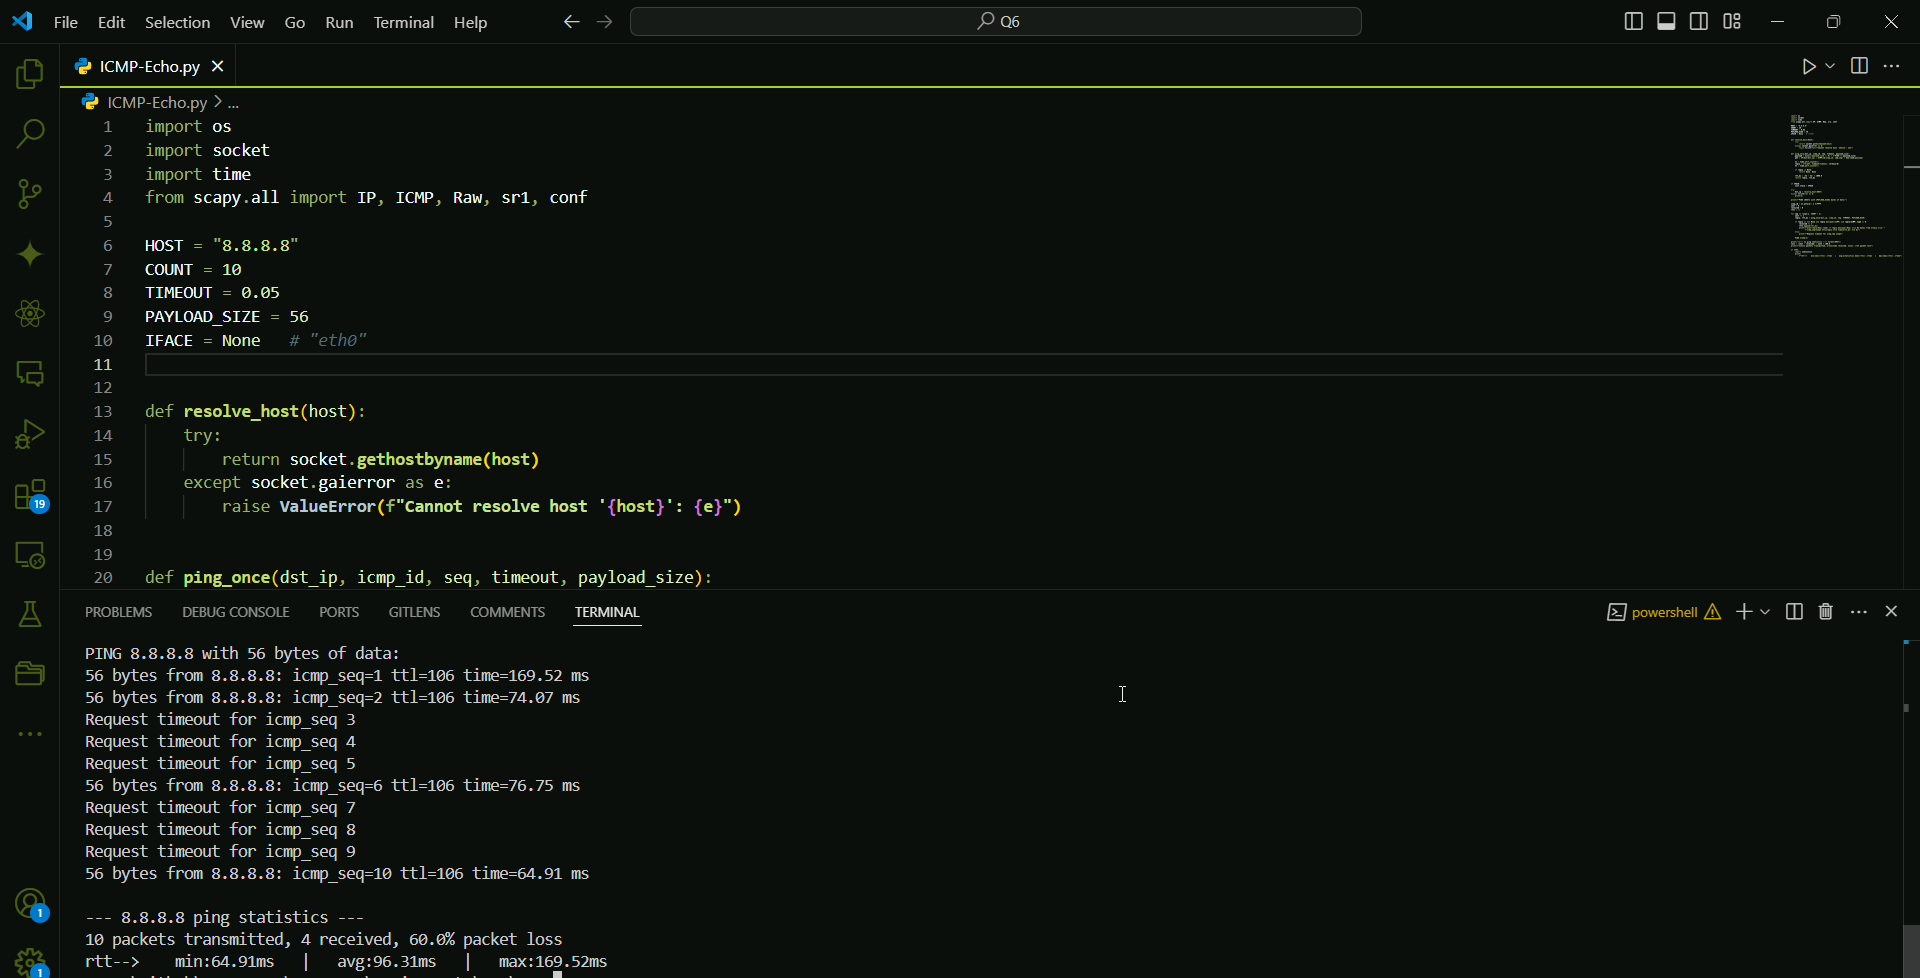
\includegraphics[width=1\textwidth]{screenshot001}
		
	}
}

پس از ارسال بسته‌ها، گزارش آماری از زمان سپری شده و تعداد بسته‌های سالم پرینت می‌شود که در تصویر فوق قابل مشاهده است.



برای تست کردن خطاهای ICMP به صورت هاردکد TTL را کم در نظر می‌گیریم تا خطای تایپ ۱۱ بگیریم.
خطا در Wireshark به این صورت نشان داده شده است:


{
	\centering{
		
		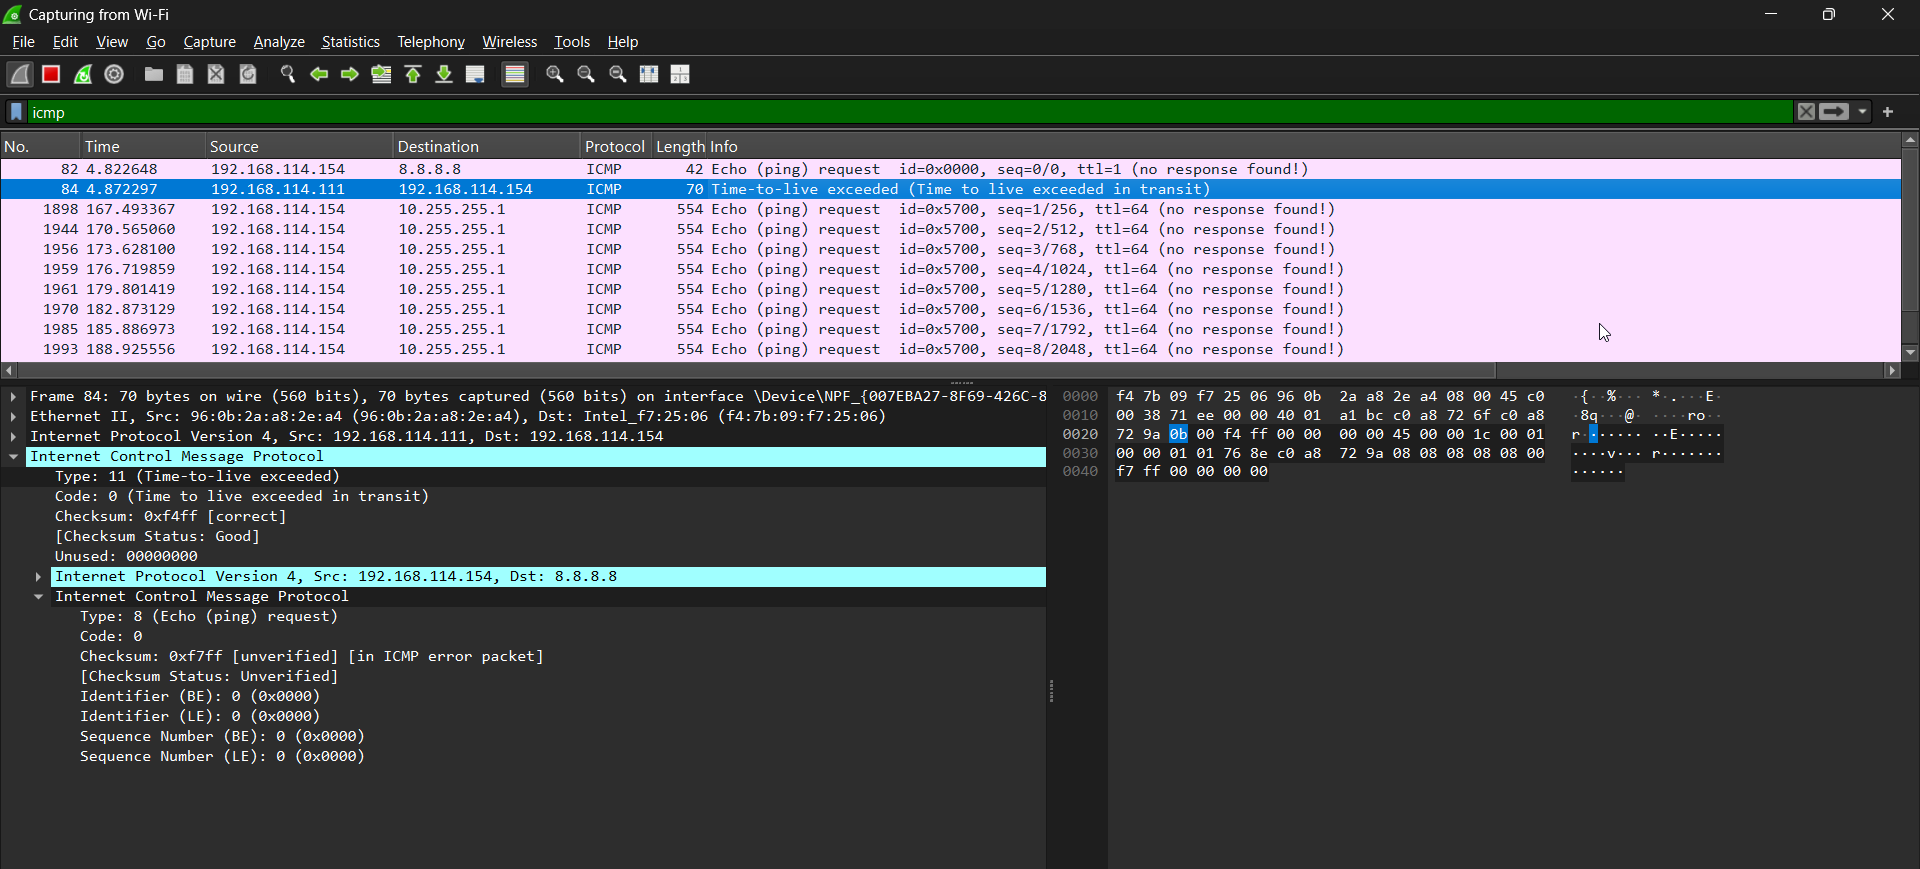
\includegraphics[width=1\textwidth]{screenshot003}
		
	}
}

\pagebreak


در ادامه توابع مهم و جزئیات پیاده‌سازی آن را مشاهده می‌کنیم:

{
	\centering{
		
		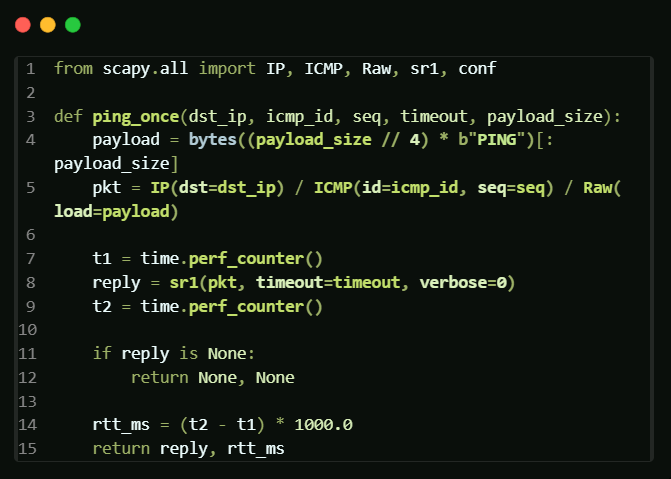
\includegraphics[width=0.5\textwidth]{screenshot002}
		
	}
}

تابع فوق که از متد‌های اماده کتابخانه
\lr{scapy}
استفاده کرده است، یک پینگ به ادرس داده شده ارسال می‌کند و RTT آن را برمی‌گرداند.


{
	\centering{
		
		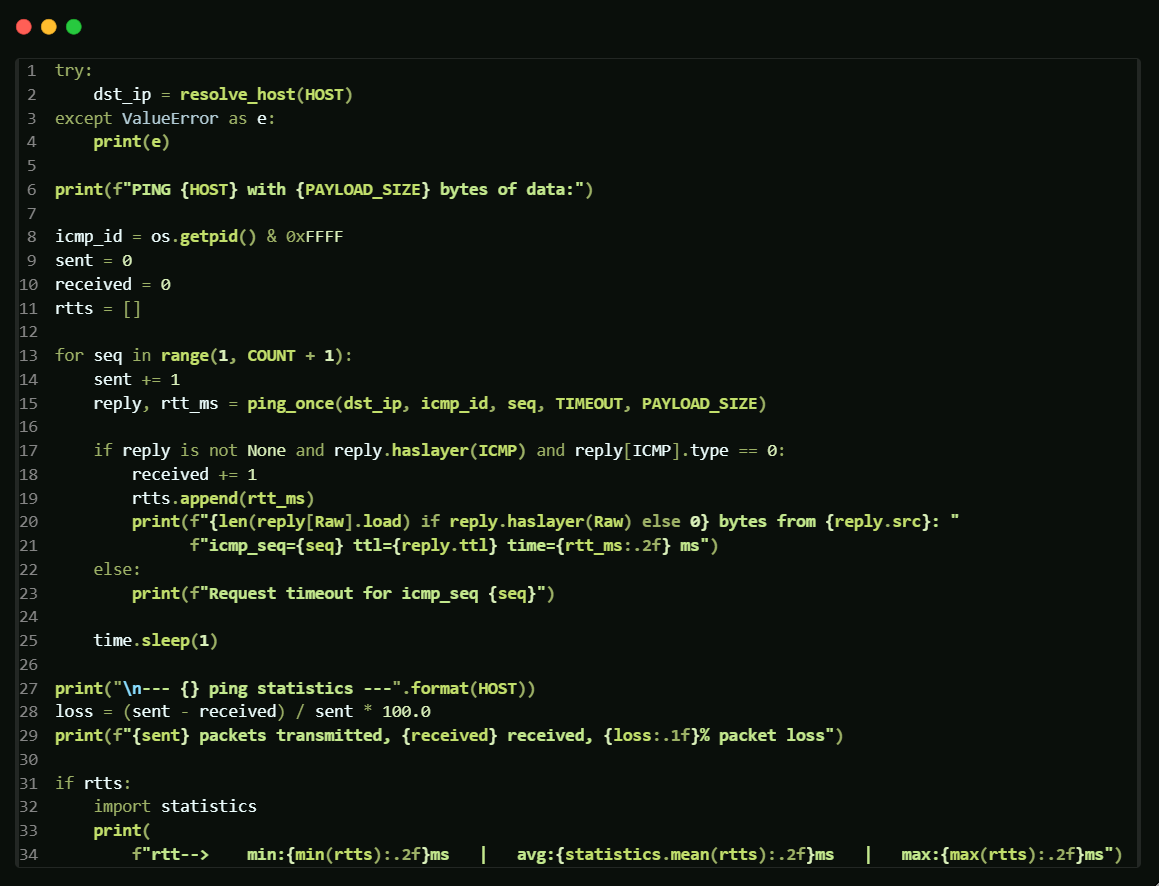
\includegraphics[width=0.75\textwidth]{screenshot004}
		
	}
}

بخش اصلی اسکریپت ما به صورت فوق است. به تعداد در نظر گرفته شده پینگ می‌کند و RTT ها را ذخیره می‌کند و در نهایت نتایج را پرینت می‌کند.

\pagebreak

\subsectionaddtolist{پیاده‌سازی برنامه Traceroute}



*****************************************************************


\subsubsection*{سوال اول - چطور روترها شناسایی می‌شوند؟}

وقتی TTL بسته شما به صفر می‌رسد، روتر بسته را دور می‌اندازد و یک
\lr{ICMP Time Exceeded}
 برای مبدا می‌فرستد. داخل این پیام، هدر IP + ۸ بایت اول
از دیتای بسته اصلی وجود دارد. از روی این اطلاعات، مبدا می‌فهمد که کدام بسته در کدام روتر افتاده و بنابراین
آدرس روتر میانی را چاپ می‌کند. به این ترتیب با \lr{TTL=1} روتر اول، با \lr{TTL=2}
روتر دوم و … شناسایی می‌شوند.

\subsubsection*{سوال دوم - چطور بعضی هاپ‌ها * می‌شوند؟}


این اتفاق دلایل مختلفی می‌تواند داشته باشد:

\begin{itemize}
	\item 
	روتر پاسخ ICMP را فیلتر می‌کند یا اصلا ICMP تولید نمی‌کند.
	\item
	بسته پاسخ در مسیر برگشت گم می‌شود یا Timeout می‌خورد.
	\item 
	فایروال در سیستم شما یا در مسیر، بسته را بلوکه می‌کند.
	\item 
	روتر آن‌قدر مشغول است که به Traceroute پاسخ نمی‌دهد.
\end{itemize}


در نتیجه در این موضوع لزومی ندارد مشکل شبکه ما و مقصد باشد؛ بسیاری از
اپراتورها عمداً پاسخ به ICMP را محدود می‌کنند.







